\documentclass{article}

\usepackage{graphicx}
\usepackage{tikz}
\usepackage{tikzsymbols}
\usetikzlibrary{calc,patterns,shapes.geometric}
\pagestyle{empty}
\usepackage[margin=0pt]{geometry}
\geometry{papersize={14in,12in}}

\def\centerarc[#1](#2)(#3:#4:#5){\draw[#1] ($(#2)+({#5*cos(#3)},{#5*sin(#3)})$) arc (#3:#4:#5);}

\begin{document}
	\begin{figure}
		\centering
		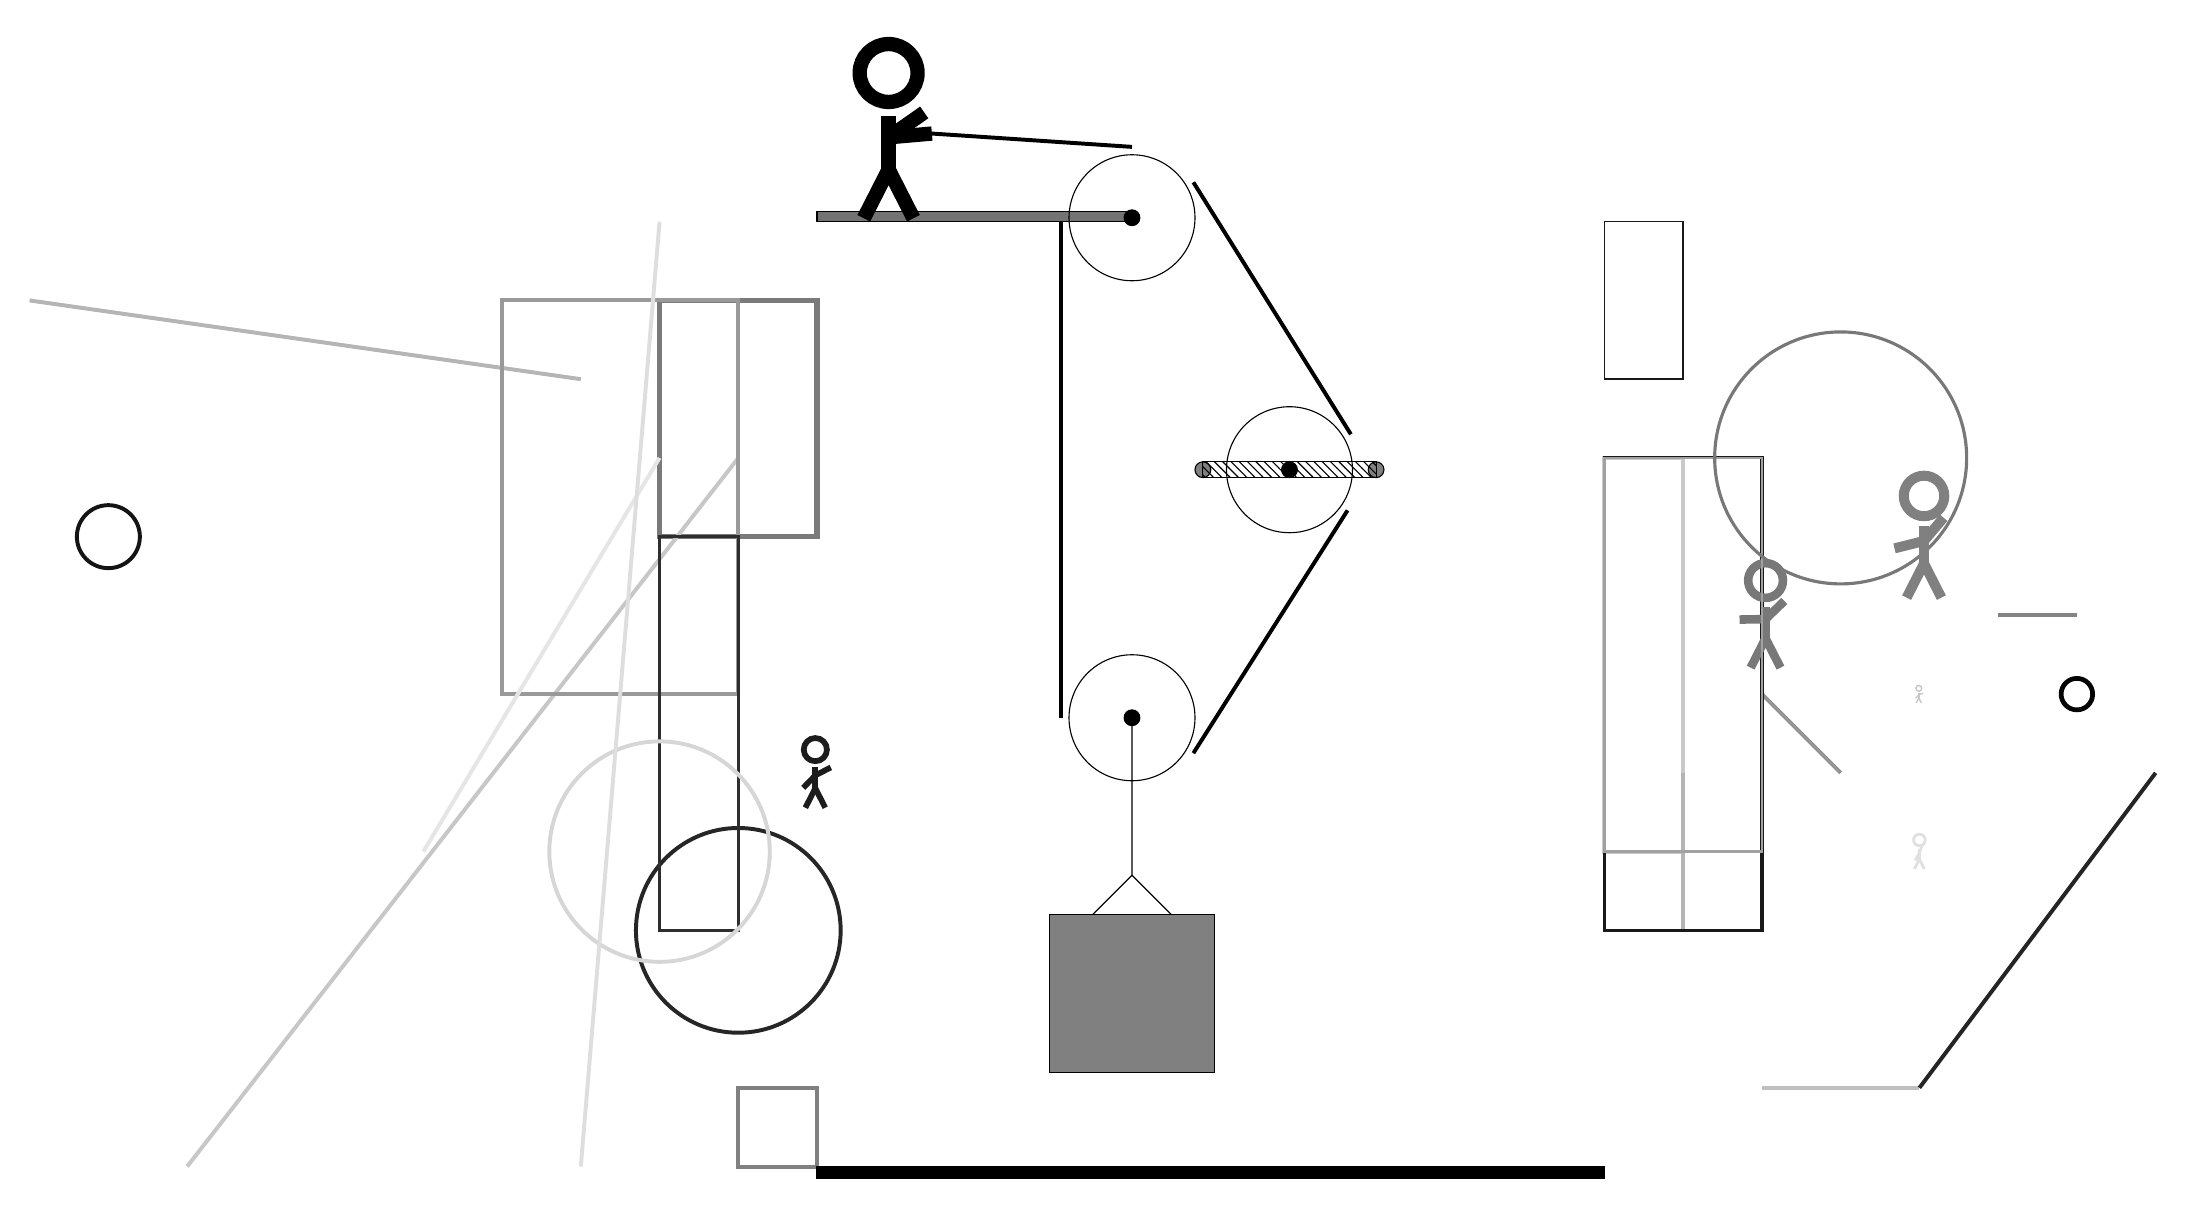
\begin{tikzpicture}
			%%%%% START %%%%%
			
			\draw[fill=black!55] (-2, 9) rectangle (2, 9.125);
			
			\draw (2, 2.7) circle (0.8);
			\draw[fill=black] (2, 2.7) circle (0.1);
			
			\draw (2, 9.05) circle (0.8);
			\draw[fill=black] (2, 9.05) circle (0.1);
			
			\draw [line width=0.5mm, color=black!85](-3, 0) circle (1.3);
			
			\draw [line width=0.6mm, color=black!99](14, 3) circle (0.2);
			\draw[line width=0.5mm, color=black!29](-5, 7) -- (-12, 8);
			\draw[line width=0.2mm, color=black!90] (9, 9) rectangle (8, 7);
			\draw[line width=0.5mm, color=black!25](10, -2) -- (12, -2);
			\draw[line width=0.7mm, color=black!52] (-2, 8) rectangle (-4, 5);
			
			\draw[line width=0.5mm, color=black!21] (8, 1) rectangle (9, 6);
			\draw[line width=0.5mm, color=black!29] (9, 2) rectangle (9, 0);
			\draw[line width=0.5mm, color=black!22](-3, 6) -- (-10, -3);
			
			\node[line width=0.5mm, color=black!12] at (12, 1) {\Strichmaxerl[2][61][70]};
			
			\draw[line width=0.5mm, color=black!42](10, 3) -- (11, 2);
			\draw[line width=0.4mm, color=black!90] (8, 6) rectangle (10, 0);
			\draw[line width=0.5mm, color=black!50] (-2, -2) rectangle (-3, -3);
			\node[line width=0.5mm, color=black!22] at (12, 3) {\Strichmaxerl[1][49][20]};
			\draw[line width=0.5mm, color=black!40] (-3, 8) rectangle (-6, 3);
			\draw[line width=0.4mm, color=black!82] (-3, 5) rectangle (-4, 0);
			\draw[line width=0.5mm, color=black!48](13, 4) -- (14, 4);
			
			\node[line width=0.6mm, color=black!53] at (10, 4) {\Strichmaxerl[6][1][44]};
			\draw [line width=0.5mm, color=black!16](-4, 1) circle (1.4);
			\draw[line width=0.5mm, color=black!86](12, -2) -- (15, 2);
			\draw[line width=0.3mm, color=black!37] (8, 6) rectangle (10, 1);
			
			\draw[line width=0.5mm, color=black!10](-4, 6) -- (-7, 1);
			\draw [line width=0.5mm, color=black!92](-11, 5) circle (0.4);
			\draw[line width=0.5mm, color=black!13](-5, -3) -- (-4, 9);
			\node[line width=0.3mm, color=black!89] at (-2, 2) {\Strichmaxerl[4][46][27]};
			
			\draw [line width=0.4mm, color=black!53](11, 6) circle (1.6);
			\node[line width=0.5mm, color=black!50] at (12, 5) {\Strichmaxerl[7][14][50]};
			\draw [line width=0.4mm, color=black!21](-5, -2) circle (0.0);
			
			\draw[fill=white](4, 5.85) circle (0.8);
			\draw[fill=black] (4, 5.85) circle (0.1);
			\draw[fill=black!50] (2.9, 5.85) circle (0.1);
			\draw[fill=black!50] (5.1, 5.85) circle (0.1);
			\draw[pattern=north west lines, pattern color=black] (2.9, 5.95) rectangle (5.1, 5.75);
			
			\draw (2, 2.7) -- (2, 0.7) -- (1.5, 0.2) -- (2.5, 0.2) -- (2, 0.7);
			\draw[fill=black!50] (0.95, 0.2) rectangle (3.05, -1.8);
			
			\draw[line width=0.5mm] (1.1, 9) -- (1.1, 2.7);
			\centerarc[line width=0.5mm](2, 2.7)(180:330:0.9);
			\draw[line width=0.5mm](2.7794, 2.25) -- (4.7373, 5.3338);
			\centerarc[line width=0.5mm](4, 5.85)(390:325:0.9);
			\draw[line width=0.5mm](4.7794, 6.3) -- (2.7794, 9.5);
			\centerarc[line width=0.5mm](2, 9.05)(30:90:0.9);
			\draw[line width=0.5mm](2, 9.95) -- (-1, 10.15);
			
			\node at (-1, 10.15) {\Strichmaxerl[10][-175][35]};
			
			\draw[fill=black] (-2, -3) rectangle (8, -3.15);
			
			%%%%% END %%%%%
		\end{tikzpicture}
	\end{figure}	
\end{document}